\documentclass{article} % For LaTeX2e
\usepackage{nips15submit_e,times}
\usepackage{hyperref}
\usepackage{url}
\usepackage{graphicx}
\usepackage{amsfonts}
\usepackage{amssymb}
\usepackage{float}
\usepackage{listings}
\usepackage{xcolor}
\usepackage{amsmath}
\usepackage[]{algorithm2e}
%\documentstyle[nips14submit_09,times,art10]{article} % For LaTeX 2.09

\usepackage[utf8]{inputenc}
\usepackage{enumerate}

\newcommand{\D}{\mathcal{D}}
\newcommand{\U}{\mathcal{U}}
\newcommand{\M}{\mathcal{M}}

\title{Predicting Publication Conference with Neural Networks}


\author{
Jingyuan Liu\\
AndrewId: jingyual\\
\texttt{jingyual@andrew.cmu.edu} \\
}


\newcommand{\fix}{\marginpar{FIX}}
\newcommand{\new}{\marginpar{NEW}}
\newcommand{\argmin}{\arg\!\min}
\newcommand{\norm}[1]{\left\lVert #1 \right\rVert}
\newcommand{\abs}[1]{\left\lvert #1 \right\rvert}
\newcommand{\inner}[1]{\left\langle #1 \right\rangle}

\nipsfinalcopy % Uncomment for camera-ready version


\begin{document}
\maketitle



\begin{abstract}
In this paper, I formulated the supervised learning framework to predict
publication conference. For this task, I explored several ways of encoding
features and introduced different classifiers. For features, I explored
meta-data feature, topic distributions, and word feature. For classifiers,
I introduced how to use Naive Bayes, Decision Tree, SVM, and Neural Networks
for this task. I evaluated different combinations of models and features with
empirical experiments. The results showed that meta-data would help improve
topic modeling features, and the best classifier is Neural Networks with
deep learning word features combined with upstream LDA topic distributions.
\end{abstract}


\section{Introduction}
% The meaning, what is the advantage of solving this problem
When researchers are composing a publication, they will decide which conference it
should be submitted to. Submitting a paper to a proper conference is of great
importance to researchers. An academic conference with related research topics
and good reputation would be likely to make the publication more influential.
Besides, conference would gather noted researchers in the filed and bring a
great opportunity to discuss about the work. Therefore, in general, submitting
publications to proper conferences would make the work more influential and
bring researchers opportunites to imporve their work.

% The motivation, how this problem came up
However, sometime it could be challenging to decide which conference should a
publication be submitted to. First of all, there are too many conferences. For
example, there are more than 120 confernces held by ACM every year. For specific filed,
like Machine Learning, besides noted ACM conferences like KDD, CIKM, WSDM, there
are many influential conferences held by other organizations like IJCAI,
ICML, and NIPS. Some regional held conferences also enjoy good reputation like
ECML and ICMLDA. Besides the scale of conference, another challenge is that some
coferences would have different subtle preferences. For example, compared with
ICML, NIPS would prefer neural and kernal related algorithms, while KDD would
prefer applications of machine learning methods on data mining. If these
challenges are well solved, we could extend the predication model to a conference
recommender system, which could be very useful, especially for those new
researchers who might get confused when deciding conference choice.

% The challenge of solving the problem
Solving this prediction problem could be challenging. At first, we would need to
encode the representative features for the whole text corpus. Good featuress are
the fundamentals for machine learning. For publication corpus, not only the words
are useful, but also the meta-data like publication authors, organizations, and
time contain very important latent information. Another challenge could be how
to choose appropriate classifiers for this task. Different classifiers are
suitable for different goals with different types of features. Most current
related works try to integrate conference information into a general topic
model. While this kind of work \cite{tang2008arnetminer} \cite{rosen2004author}
could be used to model conferences, they do not directly fall into supervised
learning framework and hardly be used for predication goal.

% The contribution of this paper
In this paper, I tried to solve these challenges and purposed a general
supervised learning framework including encoding features and building
classifiers. The main contributions are:

\begin{enumerate}[1. ]
\item I explored several different features like meta-data, topic distributions,
and word features.

\item I introduced how to do use different classifiers like Naive Bayes,
Decision Trees, SVM, and Neural Networks for predicting the publication
conference.

\item I presented empirical evluation with real-life data. I also analyzed the
results with cross validation and parameter tuning.
\end{enumerate}

The paper is organized as follows. In section 1.1, I would introduce the related
work. In section 2, I explored several different features. In section 3, I
introduced how to employ several different classifiers for the prediction goal.
In section 4, I presented the experiments and analyzed the results. In the
last section, I would conclude my work and discuss about future work.


\subsection{Related Work}
% previous modeling conference framework, A-C-T topic model
Tang proposed a variant of LDA on modeling publication conference,
academic researchers, and publications simultaneously called ACT Model
\cite{tang2008arnetminer}. This work could build conferences over hidden topics
distributions, and similar to author-topic models \cite{rosen2004author}.
Besides, there some previous work of topic modeling on integrating meta-data to
improve training performances \cite{mimno2012topic} \cite{petterson2010word}.
All these works are variants of LDA, and could be used to help model conference
and encode meta-data as features. However, they could not be directly used for
supervision tasks.

% neural networks, word2vec word features
Neural Networks are quite popular in recent days. Though not able to be well
interpreted, Neural Networks could always achieve better performances than other
classifiers. While most remarkable applications of Neural Networks are in
computer vision filed, there are still influential works used for text mining
\cite{bengio2003neural} \cite{hochreiter1997long}. Word features are useful for
modeling text, and deep learning offers another representative way of encoding
word features \cite{mikolov2013distributed}.

% other classifiers
Besides neural networks, there are some other important and useful classifiers
\cite{wu2008top} . Naive Bayes is a probabilistic generative model with assumption
that features are conditionally independent based on labels,  often used in text
classification. Decision Trees and SVM are well-performed classifiers, and
always used as baseline methods in classification tasks.






\section{Feature Engineering}
Features are the fundamentals for machine learning task. For text data, basic
features include meta-data (author, publish year, organizations), topic
distributions (latent topics of document), and word features. For different type
of features, there are different methods to transfer them to numerical values.

\subsection{Meta-data}
Meta-data is useful for modeling text. I would use index map to encode
meta-data. First of all, I would set every meta-data with a index. Then for each
publication, if the meta-data appeared, I would set the feature index as 1,
otherwise 0. Meta-data include:

\begin{enumerate}[a]
\item \textbf{Authors.} authors are very important attributes of a
paper. I can use an indicator vector to encode this attribute to a vector as
input feature. At first, I assign every different author a index. Then for each
paper, I would put 1 to the position of the index for every author in the paper,
otherwise 0.

\item \textbf{Organizations.} similar to authors.

\item \textbf{Time.} time is also very import attribute for a paper. The research
topics of a conference would change over time. Therefore, when predicting
conference for a paper, I need to take the time into consideration. I could use
the year as the input of the feature.
\end{enumerate}

\subsection{Topic Distributions}
When researchers are writing publications, they would first set the hidden topics
that publications would cover. If we could well model the hidden topic
distributions, then we could naturally model the topic distributions of
conferences via modeling publications it contained.

\subsubsection{LDA}
LDA is commonly used to mine the latent topic distributions
of documents \cite{blei2003latent} \cite{griffiths2004finding}.

\begin{figure}[!htbp]
    \centering
    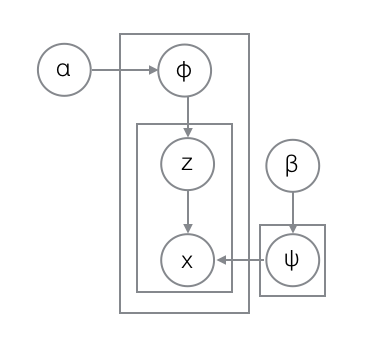
\includegraphics[width=4cm]{./pic/LDA.png}
    \caption{LDA}
\end{figure}


\begin{align*}
   & \phi_d \sim Dir (\alpha) \qquad \psi_k \sim Dir (\beta) \\
   & z_{dn} \sim Mult (\phi_x) \quad x_{dn} \sim Mult (\psi_{z_{dn}})
\end{align*}

\subsubsection{Neural Networks Upstream Conditioning LDA}
Besides traditional LDA, we could use Neural Networks Upstream Conditioning model
to mine topic distributions \cite{mimno2012topic}. The advantage of upstream
conditioning model is this method could integrate meta-data into the latent
topic distributions.

\begin{figure}[!htbp]
    \centering
    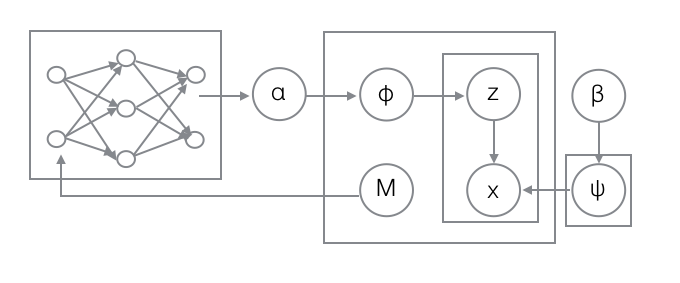
\includegraphics[width=8cm]{./pic/Up.png}
    \caption{Neural Networks Upstream Conditioning LDA}
\end{figure}

\begin{align*}
   & \alpha \sim F(M \mid W) \\
   & \phi_d \sim Dir (\alpha) \qquad \psi_k \sim Dir (\beta) \\
   & z_{dn} \sim Mult (\phi_x) \quad x_{dn} \sim Mult (\psi_{z_{dn}})
\end{align*}

\subsection{Word Features}
Word features are the most import feature for modeling documents. We have two
common ways to encode word features. The first is just use the word indicator
map, which are always used by Naive Bayes. Another way is to use word2vec, which is
a deep learning method to encode word features \cite{mikolov2013distributed}.



\section{Classification Methods}
To predict the publication conference, I formulated the supervised learning
framework to do classification. The conferences are treated as labels, and the
goal is to predict which conference a publication would belong to. Different
classifiers would have different view of this problem. I would introduce how to
use several most popular classifiers for this task.


\subsection{Scalable Smoothed Naive Bayes}
Naive Bayes is one of the most common basic classifiers with good performances.
Naive Bayes is suitable for text classification, like email spam detection
\cite{metsis2006spam}. Naive Bayes generally assumed the features are conditionally
independent over the classification labels. Therefore, with bayes rule, we could
derive:

\begin{equation*}
log P(y') = \sum_j log \frac{C (X_j=x_j \& Y=y')}{C (X=* \& Y=y')} +
log \frac{C (Y=y')}{C (Y=*)}
\end{equation*}

In general, we would add $\lambda$ smooth to avoid zero count case for Naive
Bayes. Besides, in most cases, we do not care the order of word features, which
means we would use bag of words model for Naive Bayes. With these assumptions,
we could derive:

\begin{equation*}
log P(y') = \sum_j log \frac{C(X=x_j \& Y=y')+\lambda}
{C(X=* \& Y=y') + \lambda \cdot \abs{X} } +
log \frac{C (Y=y')+\lambda}{C (Y=*)+\lambda \cdot \abs{Y} }
\end{equation*}

Naive Bayes is efficient for large scale dataset. We could use the stream and
sort pattern, which is also know as map-reduce, to make it scalable:

\begin{center}
\begin{minipage}{.75\linewidth}
\begin{algorithm}[H]
    \SetKwData{Left}{left}\SetKwData{This}{this}\SetKwData{Up}{up}
    \SetKwFunction{Union}{Union}\SetKwFunction{FindCompress}{FindCompress}
    \SetKwInOut{Input}{Input}\SetKwInOut{Output}{Output}

    \Input{Documents D with words X, and document labels Y}
    \Output{Trained Smoothed Scalabel Naive Bayes Classifier}
    \BlankLine
    \ForEach{publication with label y, and d words $x_1$, $x_2$, ...}{
        \BlankLine
        (a) Print $Y = ANY += 1$\;
        (b) Print $Y = y += 1$\;
        (c) \ForEach{word index j in 1,..d}{
                Print $Y = y \& X = x_j += 1$\;
            }
    }
    \BlankLine
    Sort the event-counter update message
    \BlankLine
    Scan and add the sorted meesage and get the final trained classifier
    \BlankLine
\caption{Scalable Smoothed Naive Bayes}
\end{algorithm}
\end{minipage}
\end{center}


\subsection{Decision Trees}
Systems that construct classifiers are one of the commonly used tools in machine
learning. Such systems take as input a collection of cases, each belonging to one
of a small number of classes and described by its values for a fixed set of
attributes, and output a classifier that can accurately predict the class to
which a new case belongs \cite{wu2008top}.

These algorithms are generally categorized as Decision Trees. Decision Trees
always achieve good performances in real-life applications. Complex decision
trees can be difficult to understand, for instance because information about one
class is usually distributed throughout the tree \cite{wu2008top}. Here we used
the C4.5 alogirithm which are implemented in Weka. C4.5 introduced an alternative
formalism consisting of a list of rules of the form “if A and B and C and ...
then class X”, where rules for each class are grouped together. A case
is classified by finding the first rule whose conditions are satisfied by the
case; if no rule is satisfied, the case is assigned to a default class
\cite{wu2008top}.


\subsection{SVM}
In today’s machine learning applications, support vector machines (SVM) are
considered a must-try. It offers one of the most robust and accurate methods
among all well-known algorithms. It has a sound theoretical foundation, requires
only a dozen examples for training, and is insensitive to the number of
dimensions. In addition, efficient methods for training SVM are also being
developed at a fast pace\cite{wu2008top}.

SVM are well introduced in Scholkopf and Smola's work \cite{scholkopf2002learning}.
Here we used the Weka SMO implementation for our task. The reason why SVM
insists on finding the maximum margin hyperplanes is that it offers the best
generalization ability. It allows not only the best classification performance
on the training data, but also leaves much room for the correct classification
of the future data \cite{wu2008top}. Besides, SVM has a good form and allows
kernelized methods which could transfer input data into a hyper space.


\subsection{Neural Networks}
Neural Networks are quite popular in recent days because of its impressively
good performances. With Neural Networks, we could both get better features and
better classifiers, although not well interpreted. While most remarkable
applications of Neural Networks are in computer vision filed, there are still
influential works used for text mining \cite{hochreiter1997long}
\cite{bengio2003neural}.

Here we just composed basic two layer neural networks since our training goal is
not very complex and the training data is not of very large scale.

\begin{figure}[!htbp]
    \centering
    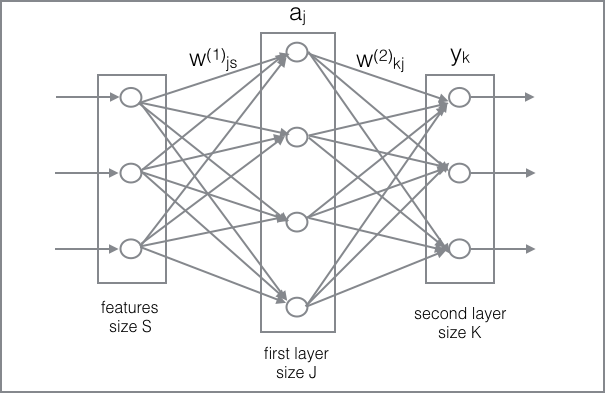
\includegraphics[width=8cm]{./pic/NN.png}
    \caption{Two Layer Neural Networks}
\end{figure}

The first layer was size J with j as index (j $>$ k).

\begin{equation}
a_{j} = \sigma (\sum_s w_{js}^{(1)} c_{s}), \qquad
\sigma (x) = \frac{1}{1 + e^{-x}}
\end{equation}

The size of second layer was K, with k as index:

\begin{equation}
y_k = \sum_j w_{kj}^{(2)} z_{j}, \qquad
\alpha_k = h(y_k)
\end{equation}

After we get $y_{k}$, we use softmax to get h for multi-label classification:

\begin{equation}
h(y_k) = \frac{e^{y_{k}}}{\sum_{k} e^{y_{k}}}
\end{equation}

The Neural Networks are implemented via mxnet, an open-source library on github.
Mxnet enables symbolic configuration, executor binding, and offers python interfaces,
which make the implementation easier.




\section{Experiments}
Here I presented a series of experiments on real-life dataset to find the best
classifiers to predict the publication conference. First I introduce my
dataset source and the cleaned data statistics. Then I showed the extracted
features. Next I explored several different classifiers to get the
best performance classifiers. At last, I would do parameter tuning for
optimization.


\subsection{Dataset}
I used the dataset from AMiner system, which is an academic social network
mining system \cite{tang2008arnetminer}. After cleaning, the whole dataset
contains over 1.5m papers. I filtered the papers in the top 10 most common
conference. The filtered dataset contains 10k publications from 10 conferences.
The dataset contains 31475 words, 5953 organizations, time ranging from 1978 to
2014. The dataset contains 14951 authors. However, most authors are sparse,
which means they would only appear once. This kind of author would not help much
in building upstream conditioning LDA model but cost much memory, therefore,
I filtered those sparse authors, and kept around 2k+ common authors for modeling.
I did similar filtering operations to organizations.



\subsection{Extracted Features}
I first presented our extracted features. Meta-data is just encoded via sparse
index matrix, with the document size times the meta-data size. Meta-data is
used as the input for Neural Networks Upstream Conditioning LDA.

\subsubsection{Topic Distributions}
I presented the topic-word distributions (top 10 words) of LDA and Neural
Networks Upstream Conditioning LDA. The above columns are the trained Upstream LDA,
and below column are the corresponding basic LDA:


% Topic 0 - Topic 4
\begin{minipage}{.196\textwidth}
\centering
\textbf{Algorithm} \\
algorithm \\
optimal \\
paper \\
set \\
based \\
graph \\
algorithms \\
proposed \\
size \\
methods
\end{minipage}
\begin{minipage}{.196\textwidth}
\centering
\textbf{Programing} \\
code \\
test \\
development \\
web \\
data \\
cost \\
cache \\
programing \\
software \\
testing
\end{minipage}
\begin{minipage}{.196\textwidth}
\centering
\textbf{Network} \\
network \\
power \\
leakage \\
energy \\
link \\
node \\
random \\
matrix \\
performance \\
communication
\end{minipage}
\begin{minipage}{.196\textwidth}
\centering
\textbf{Social} \\
social \\
human \\
link \\
clustering \\
opinion \\
society\\
network \\
user \\
algorithm \\
search
\end{minipage}
\begin{minipage}{.196\textwidth}
\centering
\textbf{Machine Learning} \\
data \\
svm \\
kernel \\
flow \\
algorithm \\
research \\
approach \\
simulation \\
environment \\
performances
\end{minipage}
% Topic 0 - Topic 4

% Topic 5 - Topic 9
\begin{minipage}{.196\textwidth}
\centering
algorithms \\
graph \\
set \\
time \\
tree \\
rate \\
paper \\
framework \\
solution \\
efficient
\end{minipage}
\begin{minipage}{.196\textwidth}
\centering
dynamic \\
computing \\
code \\
resources \\
programing \\
implementation \\
load \\
language \\
allows \\
words
\end{minipage}
\begin{minipage}{.196\textwidth}
\centering
network \\
networks \\
proposed \\
sensor \\
nodes \\
protocal \\
delay \\
layer \\
based \\
link
\end{minipage}
\begin{minipage}{.196\textwidth}
\centering
user \\
social \\
information \\
interaction \\
study \\
online \\
future \\
design \\
using \\
online
\end{minipage}
\begin{minipage}{.196\textwidth}
\centering
model \\
models \\
modeling \\
stucture \\
terms \\
svm \\
approach \\
research \\
study \\
global
\end{minipage}
% Topic 5 - Topic 9

From the top 10 words in typical Learned topics, we could see that the extracted
features are similar. Then I presented the training likelihood over iteration to
show the converge speed.

\begin{figure}[!htbp]
    \centering
    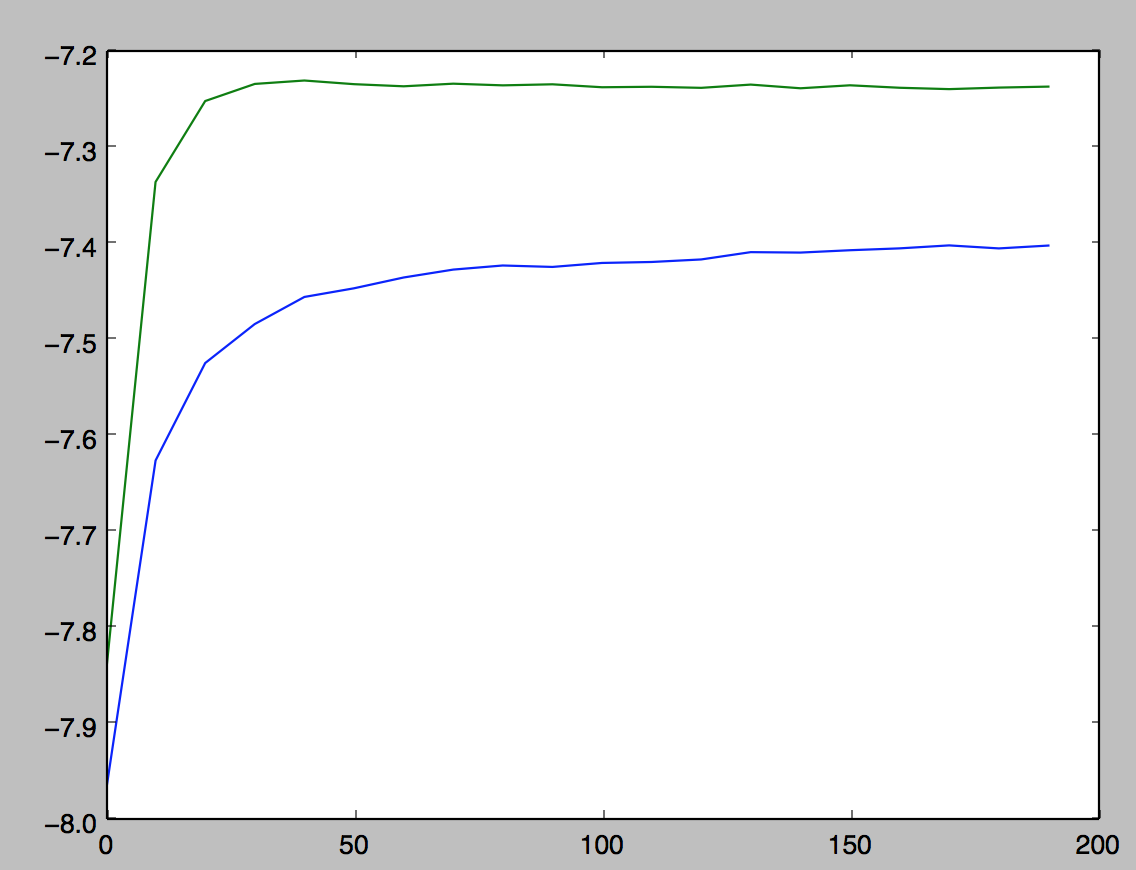
\includegraphics[width=6cm]{./pic/LLHW.png}
    \caption{Training LLHW}
\end{figure}

The green line is Upstream LDA and the bule is LDA.
We could see that the Neural Networks Upstream Conditioning LDA would achieve
higher training likelihood with faster speed. Therefore, it should be better
features that is more fitting to the data.

\subsubsection{Deep Learning Word Features}
I used the word2vec to get the Deep Learning Word Features
\cite{mikolov2013distributed}. Word2vec is famous for finding the most similar
word phrases. Here, I presented several typical similar words with cosine
similarity.


\begin{minipage}{.310\textwidth}
\centering
\textbf{Algorithm} \\
algorithms \quad 0.732173 \\
pruning \quad 0.715835 \\
method \quad 0.705341 \\
greedy \quad 0.700185 \\
heuristic \quad 0.692098\\
proposed \quad 0.687952 \\
technique \quad 0.666948 \\
iteratively \quad 0.616023 \\
tabu \quad 0.610261 \\
bisection \quad 0.607905
\end{minipage}
\begin{minipage}{.310\textwidth}
\centering
\textbf{Network} \\
networks \quad 0.825327 \\
topology \quad 0.744842 \\
wireless \quad 0.665959 \\
gateways \quad 0.657244 \\
link \quad 0.652112 \\
node \quad 0.541835 \\
topologies \quad 0.645444 \\
traffic \quad 0.639832 \\
nodes \quad 0.624277 \\
overlap \quad 0.607500
\end{minipage}
\begin{minipage}{.310\textwidth}
\centering
\textbf{Model} \\
models \quad 0.751951\\
modeling \quad 0656805\\
mathematic \quad 0.625505 \\
markov \quad 0.603707 \\
stoachastic \quad 0.603393\\
svm \quad 0.595648 \\
probabilistic \quad 0.5758 \\
lingo \quad 0.573474 \\
tree \quad 0.573412 \\
parametric \quad 0.573359
\end{minipage}

For our prediction goal, I used the doc2vec, a variant of word2vec, which could
transfer a doc to a numeric vector as our deep learning word features.

\subsection{Classification Performances}
After extracting features, we could start testing with classifiers to get the
classification performances.

First I just started with baseline methods. For baseline, I would use Scalable
Smoothed Naive Bayes, C4.5 Decision Trees, SVM implemented via SMO, and Two
Layer Neural Networks. For Naive Bayes, I used the basic word feature. For
other classifiers, I used the basic LDA topic distributions.


\begin{table}[h]
\renewcommand{\arraystretch}{1.5}
\centering
\begin{tabular}{|c|c|c|c|c|}
\hline
accuracy
& Naive Bayes
& Decision Tree
& SVM
& Neural Network \\
\hline
Training
& 0.556
& 0.633
& 0.626
& \textbf{0.643}\\
\hline
Tesing
& 0.515
& 0.605
& 0.634
& \textbf{0.645}\\
\hline
\end{tabular}
\caption{Baseline Methods with Basic Features}
\end{table}

From the above baseline method performance table, we could see with the basic
features, Naive Bayes is obviously worse than other classification methods.
Therefore, we no longer consider Naive Bayes for this task. Then I would
explored which feature would help most for prediction goal.

\begin{table}[h]
\renewcommand{\arraystretch}{1.5}
\centering
\begin{tabular}{|c|c|c|c|c|}
\hline
accuracy
& LDA
& Upstream LDA
& word2vec
& word2vec+UpLDA \\
\hline
DT
& 0.605
& 0.616
& 0.625
& 0.595\\
\hline
SVM
& 0.634
& 0.647
& \textbf{0.682}
& 0.685 \\
\hline
NN
& \textbf{0.643}
& \textbf{0.655}
& 0.678
& \textbf{0.707} \\
\hline
\end{tabular}
\caption{Test Performances with Different Features}
\end{table}

The results are showed in the table 2, which recorded the test performances for
each classifiers. From the table, we would know that in most cases, NN would be
the best choice for prediction goal. Besides, we would find that the best
feature is to combine Neural Networks Upstream Conditoning LDA feature, which are
trained with meta-data beyond basic topic distributions, and Deep Learning Word
Features, the word2vec. Another interesting fact is when combining UpLDA and
word2vec as feature, Decision Trees would get lower performances. This could be
that Decision Trees are always not scalable and tend to be overfitting with
large scale feature vector.

\subsection{Parameter Tuning for Optimization}
After finding the best classifier and best feature, then I do parameter tuning
for optimization. The basic parameter for NN is the number of hidden points in
the hidden layers. Basically, the more hidden points, the complex the model is.
For my Neural Networks, there are two layer, the second layer size was set to
10, which is the label size. So I tuned the first hidden number, ranging from
100 to 500, and got the results.


\begin{figure}[!htbp]
    \centering
    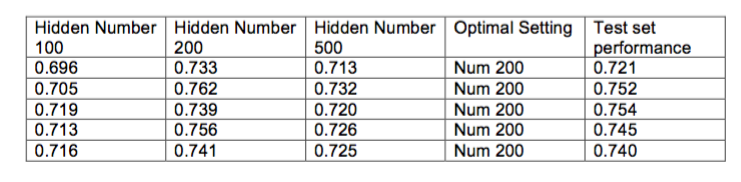
\includegraphics[width=14cm]{./pic/Result.png}
    \caption{Parameter Tuning}
\end{figure}

From the figure above, we would see that the Hidden Number = 200 would get the
best performances. Setting Hidden Number = 500 would be overfitting, which means
we are trying to use a too complex model to fit a comparatively simple dataset.




\section{Conclusion and Future Work}
In this paper, I formulated the supervised learning framework for predicting
the publication conference. I explored several ways of encoding the publication
information as features. I also discussed about several common and powerful
classifiers for classification. After a series of experiments and
parameter tuning. I found that the Neural Networks would achieve best
performances. The best feature should be the Deep Learning Word Features
combining with Neural Networks Upstream Conditioning LDA topic distributions.
The best parameters for the model should be 200 hidden nodes for the first
layer.

The future work mainly falls into two parts, the first is to extract features in
a more elgant way. From current result, I could see that the topic distributions
and word features are two different aspects of view on representing dataset and
could help each other. However, I just arbitraryly combine these two features.
Another point is how to overcome overfitting. We could see the results are
sensitive to the number of hidden nodes. And after combining two features, the
input feature size could be very big, thus might lead to overfitting for some
sensitive classifiers like Decision Trees.




\bibliography{mybib}{}
\bibliographystyle{plain}


\end{document}
